\documentclass[11pt]{article}
\usepackage{acl2014}
\usepackage{times}
\usepackage{url}
\usepackage{graphicx}
%\usepackage{latexsym}


%figures:
\usepackage{tikz}
\usetikzlibrary{trees,positioning,backgrounds}
%\usepackage{tikz-qtree}
\usepackage{subcaption}

%references and keeping floats in place
\usepackage[pdftex,pdfborder={0 0 0},unicode,breaklinks,hyperfootnotes=false,bookmarks]{hyperref}
\usepackage[section]{placeins}

\usepackage{amsmath} 
\renewcommand{\vec}[1]{\mathbf{#1}}

\title{Statistical Structure in Language Processing \\Using multi-parallel data for phrase-table improvement}
\author{ Cristina G\^arbacea\\
  10407936 \\
  {\small \tt cr1st1na.garbacea@gmail.com} 
  \\\And
  Sara Veldhoen \\
10545298   \\
  {\small \tt sara.veldhoen@student.uva.nl} \\}

\date{}

\begin{document}

\maketitle

\begin{abstract}
In this paper we continue to extend upon our previous assignment by building a phrase pair extraction tool that would use evidence from aligned parallel corpora. Unlike in our previous work where we would only use parallel corpora consisting of two languages, this time we use evidence from multilingual parallel aligned corpora made available by Europarl. We investigate how word alignments between several languages can be of use in extracting consistent phrase pairs. %along with their conditional and joint probabilities 
%and consider how word alignment symmetrization can be improved from multilingual word alignments of the same target sentence. 
We present an algorithm to do so, and experimented with different symmetrization heuristics to be used as an input. Furthermore, we investigated how the choice of reference languages influences improvement. We compare our results to a baseline system, and to a different approach to phrase table filtering, based on significance testing.
\end{abstract}

\section{Introduction}
Phrase-based statistical machine translation relies on estimates of translation probabilities for pairs of phrases, stored in a so-called phrase table.
In principle, the set of possible phrase pairs is far too huge to be computationally manageable, especially if the size of the corpus grows.
Therefore, we need to restrict this set in some way, to keep only useful/ meaningful phrase pairs. This reduction might be the main challenge in phrase based machine translation.

In the approach we took in the previous assignment, the reduction was based on Giza++ output: only those phrase pairs that were consistent with symmetrized word alignments were added to the phrase table. This is a standard approach, that yields a large reduction and proves useful for translation, obtaining for instance a BLEU score of 24.68 in our previous assignment \cite{previous}.
%But the MT community has moved forward, and can do better now.

The possibility that we aim to investigate in this project, is to use multi-parallel corpora. These data consist of documents in more than two languages with aligned sentences. The process of incorporating evidence from multilingual data in a single system is called \emph{triangulation}, and presents the advantage of using a wider range of parallel corpora for training. 

\section{Related work}

%Johnson
In \cite{Johnson} the bulk of phrase table is reduced based on the significance testing of phrase pair co-occurrence in the parallel corpus. The authors present two methods of testing the significance of associations in two by two contingency tables departing from calculating the probability that the observed table can occur by chance assuming a model of independence. For this purpose they use Chi-squared and Fisher exact test and experiment with different pruning threshold values ranging between 14 and 25. They outline that while the savings in terms of number of phrases discarded are considerable, the translation quality as measured by the BLEU score is preserved, and even more surprisingly it can even increase as compared to the case when all phrase pairs are kept. This makes their approach a valuable contribution to the field of machine translation.


%Chen, Eisele and Kay 
In contrast to the approach described above, \cite{chen} does use triangulation to reduce the phrase tables.
Two methods are presented to filter the phrase table for a language pair, based on an intermediate third \emph{bridge} language. Both methods assume an existing {\em source-target} phrase table, based on Giza++, and filter its entries with evidence from phrase tables {\em source-bridge} and {\em bridge-target}.

In method 1, for each phrase pair $\langle s, t\rangle \in source-target$, it is kept if there is an entire phrase $b$ in the bridge language such that $\langle s,b\rangle \in source-bridge$ and also $\langle b,t\rangle \in bridge-target$.

Method 2 is somewhat more lenient, in that it looks at the words occurring in the phrases instead of an exact match of the entire phrase. An overlap score is assigned to each phrase pair, based on the intersection of the vocabularies in the phrases. The filtering is done by placing a threshold on this score.

% Cohn and Lapata
The authors of \cite{cohn} focus less on reducing the phrase tables, but use triangulation to obtain high quality phrase tables from multilingual data, even if they are not from the same corpus. They use a summation over several intermediate languages to form a probability estimate: $p(s|t)=\sum_i p(s|i)p(i|t)$. Interestingly, the triangulated phrase table is trained separate from the standard phrase table, so that it can be used as a distinct feature in decoding.


%\section{Goals}
%In this project we are planning to build a phrase pair extraction tool for phrases of up to length 7 that would use evidence from multilingual aligned corpora. To achieve our goal we aim to use Europarl % cite EUroparl
%data for Dutch, English, Romanian, French, German. % maybe add some more?
%We are planning to investigate how we can use the evidence from word alignments between several languages to extract, rather than filter, phrase pairs and estimate their conditional and joint probabilities. For this, we consider the possibility to improve word alignment symmetrization from multilingual word alignments of the same target sentence.

\section{Our approach}
We use evidence from multiparallel data in the process of phrase extraction, rather than filter the phrase tables as described in \cite{chen}. We extended a simple phrase extraction algorithm with a sanity check on possible English windows. An (English) phrase, we imagine, is only a meaningful whole if it has a consistent translation in other languages. We therefore discard all English windows that do not have a consistent foreign window in any of the reference languages.

\begin{figure*}[t]
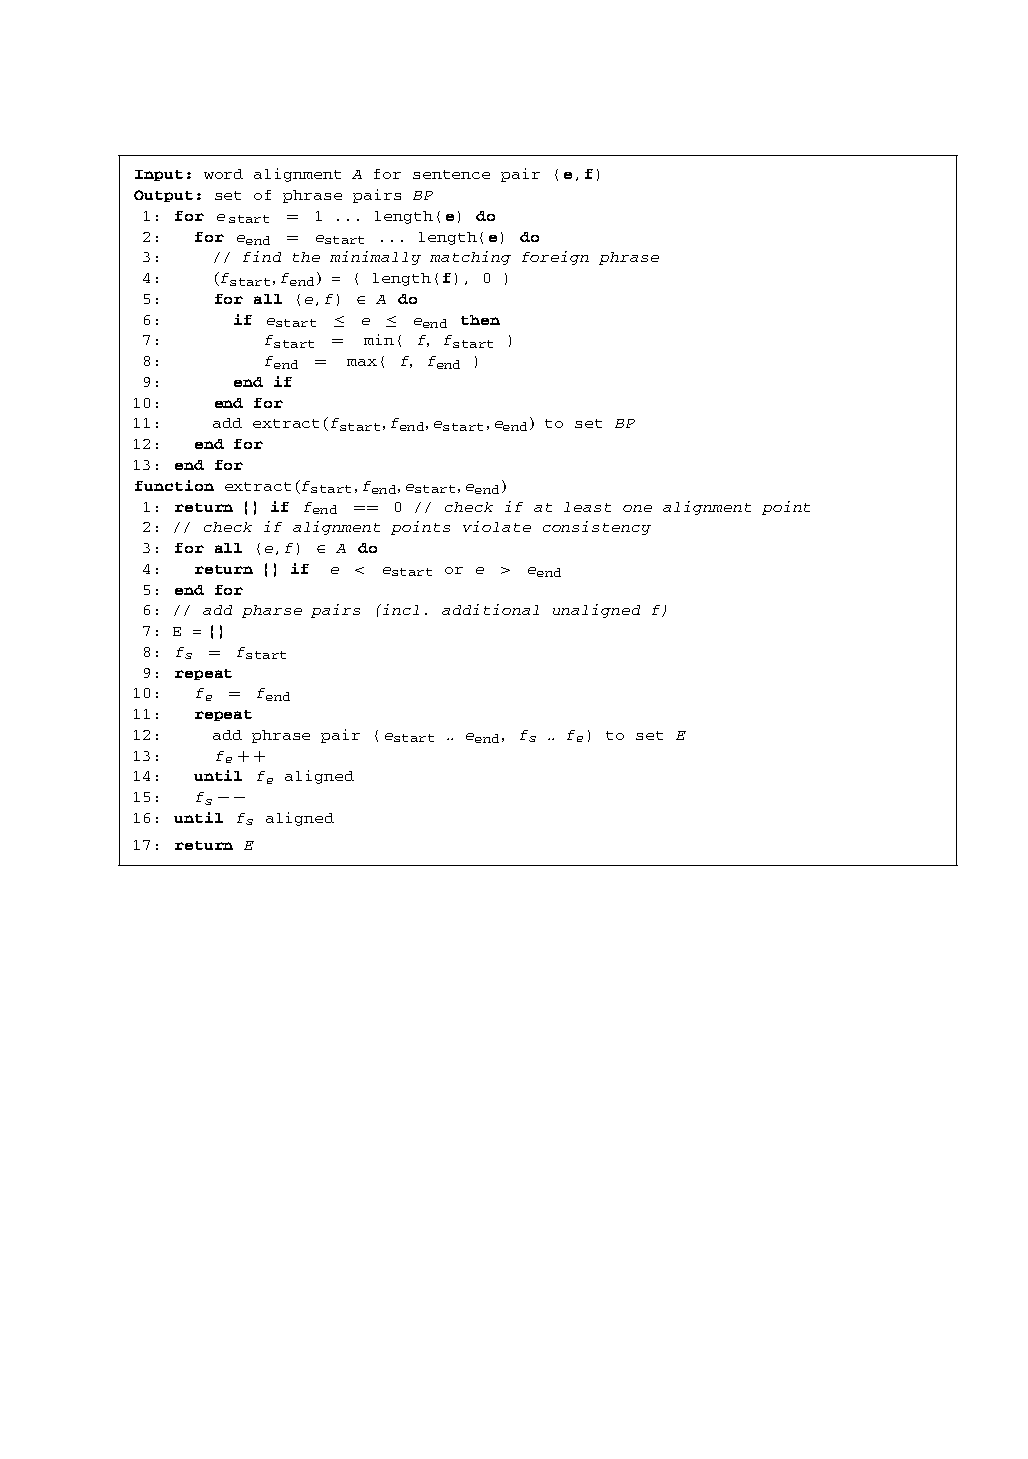
\includegraphics[width=\textwidth]{koehnExtractionAlgorithm}
\caption{Phrase extraction algorithm, reproduced from \protect\cite{Koehn:2010}}
\label{f:algorithm}
\end{figure*}

Although we changed some implementation details, our algorithm is essentially similar to the one described in \cite[page 133]{Koehn:2010}, as reproduced in figure \ref{f:algorithm}. Our extension adds a check after line 2, that the English window be consistent with some window in each reference foreign alignment.



\subsection{Multi-parallel data}

The parallel data is sentence aligned, which means that each line in the source text corresponds to a line in the target text.
In order for our phrase extraction to work, we want one single English (target) text file to be aligned to all languages.

Our implementation is quite ad hoc, in that it compares the English sides and just discards those lines that are different. This means we discard part of the data, because in the original parallel data sometimes multiple sentences are concatenated in the sentence alignment. This approach could probably be refined to lose less data, but due to time constraints and memory efficiency reasons we preferred to keep only those lines that are common in all English files. 

In what follows we describe our sentence alignment approach. From all the English files in the list of parallel data that we have for the 7 language pairs, we pick one randomly (we chose the English file from the English - Danish corpus in this case) and we retain only those sentences that are present in the other English files belonging to the other corpora. In this way we aim to identify common English sentences in all English files from the parallel corpora that we have. For each such sentence found we preserve the index of the occurrence so that we can retrieve its corresponding translations in the foreign languages we use. Usually these indices will denote the position of the corresponding translated sentence inside the foreign files. However, we are aware that this will not always be the case. For computation efficiency reasons, instead of looping though all the lines in a foreign file in searching for the translated version of the English sentence, we prefer to keep track of the last retrieved position $i_l$ from the English file and count the number of lines $n_s$ skipped since then to look up the corresponding foreign phrase within a window ranging between $i_l$ and $100 + i_l + n_s*2$. We chose to add 100 and multiply $n_s$ by 2 as a safe margin leaving from the premises that we should include in our search all the sentences located in the neighborhood of the expected index. 
The output of our preprocessing algorithm consists in the English file having only the common sentences and the 7 foreign files for each of the different languages we use containing the corresponding versions of the English sentences which are now properly aligned with our English sentences. 

\subsection{Word-alignments}
 The consistency of a phrase pair is based on symmetrized Giza++ word alignments.

The bidirectional word alignments are obtained with {\tt Giza++}, which is a combination of IBM-models. Although the quality of these alignments is not very high on itself, they have proven to be a useful guide in the extraction of phrase pairs. 

%The symmetrization is done by Moses, which provides several heuristics to do so. We use the default setting for our baseline, i.e. grow-diag-final-and. 

 Because of the design of IBM models, the Giza word-alignments are one to many. For symmetrized word alignment, where many-to-many alignments are possible, Giza alignments for both directions are used and their alignment points combined. Each word-alignment can be viewed as a matrix with words in both languages along the axes, and binary values in the cells: either the words are aligned, or not. 

The Moses alignment symmetrization is aimed to recast two such matrices back into a single binary matrix. 
Moses provides several heuristics for this step:\begin{itemize}
\item {\tt union} contains alignment points from either matrix. This heuristic has a high recall, but might have many false positives.
\item  {\tt intersection} keeps only the points that occur in both matrices. These are the high-confidence points, thus improving precision but (generally) dropping recall.
\item {\tt grow} starts from the intersection and adds block-neighboring non-empty cells.
\item {\tt grow-diag} is like {\tt grow}, but it also includes diagonally neighboring non-empty cells.
\item {\tt final} is used after either heuristic, to add as many as possible unaligned words that are not neighbored.  %Don't fully understand how though. This intruduces the resumed-unterbrochene alignment in the example
%\item {\tt grow-diag-final-and} is not explained in the Moses manual
\end{itemize}

Since the symmetrized alignments are used for reducing the space of phrase pairs, having less alignment points, as in the intersection heuristic, is actually the more lenient choice for the phrase extraction step: you do not discard phrase pairs based on weak evidence. 

The grow-diag-final is a nice midway between union and intersection, and indeed helps us reduce the phrase table without dropping phrase table quality. Our extension uses this heuristic for the symmetrized alignments of the focus language. However, we also use symmetrized alignments of the reference language sentences, to check the English window. We aim to investigate the effect of the symmetrization heuristic used for the reference languages on the size and quality of the resulting phrase table.

\section{Experiments}
We use French as the focus language in all or experiments, that is, we are translating from French to English. 

As a baseline, we run Moses with the same alignments that we use for the focus language in our experiments. We also compare to the Johnson phrase table reduction that was implemented into Moses.

In our first experiment, we investigate the effect of symmetrization heuristic for the reference languages. We run the extended phrase extraction algorithm with union, intersection, and grow-diag-final symmetrized word alignments. The reference languages used in these experiment are Italian and Dutch.

 In our second experiment, we explore the effects of choosing certain languages as reference. As a reference, we use either languages that are very similar (Italian and Spanish) or very different (Danish and Dutch) from the focus language. We expect the latter set of languages to provide more useful evidence, as their word order will be more distinct and therefore more informative as to whether an English window is sensible.

Furthermore, we conduct one experiment with just very many reference languages (Danish, Dutch, German, Italian, Portuguese, and Spanish). More languages means more evidence, so a further reduction of the phrase table. We try to investigate whether the quality is kept up. 


\subsection{Methodology}

We run Moses steps 1 and 2 with default setting on all language pairs to obtain the \textit{Giza} word alignments, taken from the intersection of bidirectional runs of \textit{Giza++} and some additional alignment points from the intersection of the two runs. For each language pair we create a special structure inside our experimental results directory, i.e. the \textit{corpus} and \textit{giza} folders generated by Moses as output of these first two steps include folders specific to each language pair. After the word alignments are generated, we conduct the symmetrization step of the alignments by experimenting in turn with the \textit{intersect}, \textit{union} and \textit{grow-diag-final} heuristics, which yield 3 different types of symmetrized alignments inside our \textit{model} folder. 

For the baseline, we continue to train the SMT system with the symmetrized alignments, with the rest of the Moses steps from 4 to 9. Once the training is completed, we ask our system to translate from each foreign language that we include in our triangulation approach into English and score these translations by computing their corresponding \textit{BLEU} score. 
% Why? We would just do grow-diag-final for a baseline, and only french to english? 
%I moved the results to the results section

For the Johnson reduction, we wanted to test how pruning the phrase table with different thresholds and keeping only those significant phrase pairs can influence in a positive or negative way our previously obtained results. In this respect we make use of the threshold-filter.perl script which we supply with values ranging between 0.001, 0.1, 0.9, \ldots. Increasing the threshold value is equivalent to dropping more phrase pairs that present less relevance. We feed the reduced phrase table back to Moses and train the SMT system starting with step 6 for scoring phrases. We ask Moses to translate our test set sentences and we score these translations using the BLEU metric.  We test according to the \textit{grow-diag-final} heuristic, the one which gave the best results so far.
%I moved the results to the results section

For our own experiments, we use the symmetrized alignments to extract phrases with our extended algorithm, with the different experimental settings described above. We evaluate by computing coverage as compared to held-out data, see below. We also use the best scoring phrase tables to decode the test data and compute BLEU scores.


\subsection{Data}

We use the Europarl version 7 parallel data for English to respectively French, German, Danish, Italian, Dutch, Spanish, and Portuguese. This choice was based on the fact that parallel data exists for parliament proceedings of the same time interval for these languages, so that they are in a sense parallel beyond language level.
We excluded Greek because of the following remark: ``Some recent Greek data has only parts of transcripts in the files." Moreover, the Greek data was not in a readable format, because of the deviant alphabet.

We use a script that comes with the Moses installation for initial preprocessing. It discards empty lines and lines with sentences that exceed a length threshold. Furthermore, all text is lowercased.

The Europarl recommends to set aside the Q4/2000 portion of the data for testing. However, the clean parallel corpora don't have time annotation, so there is no easy way to make this split. Therefore we decided to just create a split ourselves. Each $50^{th}$ sentence is removed from the corpus and added to a separate test file. The ratio is based on the fact that the Q4/2000 portion would be $\frac{3}{16*12-4}=0.016$ of the data. For the held-out/ training split, we use the same procedure.



\subsection{Evaluation}
Since our algorithm is aimed at reducing the phrasetables, we compare the size of the phrase tables for all the experiments we conduct. Furthermore, we want to measure the quality of the phrase tables.

The baseline and Johnson trained systems are used for decoding a test set. The BLEU scores are computed with the single reference translation form the Europarl data.

Decoding and computing BLEU score are quite intensive, so we choose to not follow this procedure for all our experiments. Instead, we compute the coverage of the phrasetables with respect to a held-out set. We first train Giza++ on the entire training data, to obtain the Viterbi word alignments. Then we split both the corpus and corresponding symmetrized alignments into a train and held-out set. We extract a phrase table from both sets with identical experiment settings, and determine the percentage of phrase pairs in the held-out phrase table that occurs in the training phrase table. 

Although a bit rough, we believe this is indicative of the usefulness of the phrase table for unseen data. The best scoring phrase tables from each experiment are then used for decoding to obtain a BLEU score that can be compared to the baseline and Johnson system. 

%\newpage


\section{Results}

After running our preprocessing script, to align the sentences form different language pairs, we managed to get a number of 73.872 sentences inside each file. 2\% of the data is set aside for testing.


%Size of the phrase tables for different settings

%Coverage

%BLEU Scores = decoding performance
In Table \ref{bleuGrowDiagFinal}, \ref{bleuUnion}, \ref{bleuIntersect} inside the Appendix we report our baseline results for each of the symmetrization heuristics previously mentioned. We observe that despite of the fact that the scores are lower than we expected them to be, possibly because of some alignment points out of range, the \textit{grow-diag-final} heuristic is constantly outputting the most accurate \textit{BLEU} scores.

 Just as in \cite{Johnson}, our results confirm that the quality of the translation remains unaffected when we filter with a 0.001, 0.1, 0.9 threshold the total number of phrase pairs. 


\begin{table*}[t]
\center
\begin{tabular}{p{.3\linewidth} | c c c }
&Size& Coverage & BLEU \\\hline\hline
Baseline &1995778&&13.12	\\
Johnson, threshold = 0.01&1380472&&13.12	\\\hline
union		\\
intersect	\\
grow-diag-final	\\\hline
Similar reference languages	\\
Different reference languages 	\\
All reference languages		\\\hline
\end{tabular}

\caption{Experimental results, focus language is French, target language is English. Size is the number of phrase pairs in the phrase table, Coverage the percentage of phrase pairs in a held-out phrase table in the corresponding training phrase table, BLEU the decoding performance.}
\end{table*}




%Idea: only use pruned data for extraction - prevent sparsity
%Relative size of the data after preprocessing


\section{Conclusion}

% Future: apllicable for parallel data from different domains, so not language-parallel (is that possible?)
A major drawback of our approach is the constraint that the multi-parallel corpus has to be aligned, so that the target-sides coincide. Apart from the possibility to improve the tool for extracting such data from a corpus like Europarl, it may be interesting to investigate the possibility to abandon this constraint at all. For instance, by using an existing (bilingually trained) system to provide translations for the English sentences in other languages. This would however severely aggravate the training of the model, so the question is whether the reduction in phrase table expected from our method is worth it.
%We can say more about this once we actually have results..


\begin{thebibliography}{}

\bibitem[1]{previous}
{Cristina G{\^a}rbacea and Sara Veldhoen},
\newblock{2014}.
\newblock{\em Phrase based models},
\newblock Statistical Structure in Language Processing assignment

\bibitem[2]{Johnson}
{J Howard Johnson, Joel Martin, George Foster and Roland Kuhn},
\newblock{2007}.
\newblock{\em Improving Translation Quality by Discarding Most of the Phrasetable},
\newblock {In Proceedings of EMNLP-CoNLL}

\bibitem[3]{chen}
{Yu Chen, Andreas Eisele, Martin Kay},
\newblock{2008}.
\newblock{\em Improving Statistical Machine Translation Efficiency by Triangulation},
\newblock LREC

\bibitem[4]{cohn}
{Trevor Cohn and Mirella Lapata},
\newblock{2007}.
\newblock{\em Machine translation by triangulation: Making effective use of multi-parallel corpora},
\newblock {ANNUAL MEETING-ASSOCIATION FOR COMPUTATIONAL LINGUISTICS}

\bibitem[5]{Koehn:2010}
Philipp Koehn,
\newblock 2010.
\newblock {\em Statistical Machine Translation}.
\newblock Cambridge University Press.

%%\bibitem[\protect\citename{Gusfield}1997]{Gusfield:97}
%%Dan Gusfield.
%%\newblock 1997.
%%\newblock {\em Algorithms on Strings, Trees and Sequences}.
%%\newblock Cambridge University Press, Cambridge, UK.
%
%\bibitem[1]{Koehn:2010}
%Philipp Koehn,
%\newblock 2010.
%\newblock {\em Statistical Machine Translation}.
%\newblock Cambridge University Press.
%
%\bibitem[2]{marcu2002}
%{Daniel Marcu and William Wong},
%\newblock 2002.
%\newblock {\em A phrase-based, joint probability model for statistical machine translation}.
%\newblock {Association for Computational Linguistics}.
%%@inproceedings{marcu2002phrase,
%%  title={A phrase-based, joint probability model for statistical machine translation},
%%  author={Marcu, Daniel and Wong, William},
%%  booktitle={Proceedings of the ACL-02 conference on Empirical methods in natural language processing-Volume 10},
%%  pages={133--139},
%%  year={2002},
%%  organization={Association for Computational Linguistics}
%%}
%
%\bibitem[3]{och1999}
%{Franz Josef Och, Christoph Tillmann, and Hermann Ney},
%\newblock 1999.
%\newblock {\em Improved alignment models for statistical machine translation}
%\newblock {Proceedings of the Joint SIGDAT Conf. on Empirical Methods in Natural Language Processing and Very Large Corpora}.
%
%\bibitem[4]{mosesurl}
%{Koehn, Philipp},
%\newblock 2014.
%\newblock {\em Statistical Machine Translation System. User Manual and Code Guide}
%\newblock {\url{http://statmt.org/moses/manual/manual.pdf}}.
%
%\bibitem[5]{moses}
%{Koehn, Philipp, et al}
%\newblock{2007}
%\newblock{\em Moses: Open source toolkit for statistical machine translation}.
%\newblock{Proceedings of the 45th Annual Meeting of the ACL on Interactive Poster and Demonstration Sessions}.
%
%\bibitem[6]{giza++}
%{Franz Josef Och and Hermann Ney}
%\newblock{2003}
%\newblock{\em A Systematic Comparison of Various Statistical Alignment Models}.
%\newblock{Computational Linguistics, 1:29, 19-51}.
%
%\bibitem[7]{srilm}
%{Andreas Stolcke}
%\newblock{2002}
%\newblock{\em SRILM - An Extensible Language Modeling Toolkit}.
%\newblock{901--904}.
%
%\bibitem[8]{bleu}
%{Kishore Papineni and Salim Roukos and Todd Ward and Wei-Jing Zhu}
%\newblock{2002}
%\newblock{\em BLEU - A Method for Automatic Evaluation of Machine Translation}.
%\newblock{Proceedings of the 40th Annual Meeting of the Association for ACL}.
%\newblock{311--318}.


\end{thebibliography}

\newpage
\appendix
\section{Appendix}

\begin{itemize}

\item \textbf{Alignment type: grow-diag-final}
\begin{center}
    \begin{tabular}{ | l | l |}
    \hline
    \textbf{Language} & \textbf{BLEU} \\ 
    \hline
    \textit{Danish} & \textit{Score}: 1.56 \\
    & 1-gram precision: 18.1 \\
    & 2-gram precision: 2.5 \\
    & 3-gram precision: 0,7 \\
    & 4-gram precision: 0,4 \\
    & BP$=$0.813 \\
    & ratio$=$0.829 \\
    & hyp$\_$len$=$26.953 \\
    & ref$\_$len$=$32.526\\
    \hline
    \textit{Deutsch} & \textit{Score}: 0? \\
    \hline
    \textit{Spanish} & \textit{Score}: 13.51 \\
    & 1-gram precision: 44.4 \\
    & 2-gram precision: 20.2 \\
    & 3-gram precision: 12.2 \\
    & 4-gram precision: 8.0 \\
    & BP$=$0,786 \\
    & ratio$=$0,806 \\
    & hyp$\_$len$=$26.215 \\
    & ref$\_$len$=$32.526\\
    \hline
    \textit{French} & \textit{Score}: 13.12 \\
    & 1-gram precision: 43.4 \\
    & 2-gram precision: 19.4 \\
    & 3-gram precision: 11.1 \\
    & 4-gram precision: 7.0 \\
    & BP$=$0,820 \\
    & ratio$=$0,834 \\
    & hyp$\_$len$=$27.137 \\
    & ref$\_$len$=$32.526\\
    \hline % split table here
    \textit{Italian} & \textit{Score}: 12.77 \\
    & 1-gram precision: 41.8 \\
    & 2-gram precision: 18.7 \\
    & 3-gram precision: 11.5 \\
    & 4-gram precision: 7.8 \\
    & BP$=$0,787 \\
    & ratio$=$0,807 \\
    & hyp$\_$len$=$22.236 \\
    & ref$\_$len$=$32.526\\
    \hline
    \textit{Dutch} & \textit{Score}: 10.95 \\
    & 1-gram precision: 39.5 \\
    & 2-gram precision: 16.3 \\
    & 3-gram precision: 9.0 \\
    & 4-gram precision: 5.7 \\
    & BP$=$0,813 \\
    & ratio$=$0,829 \\
    & hyp$\_$len$=$26.955 \\
    & ref$\_$len$=$32.526\\
    \hline
    \end{tabular}
    
    \begin{table}
    \begin{tabular}{ | l | l |}
    \hline
    \textbf{Language} & \textbf{BLEU} \\ 
    \hline
    \textit{Portugese} & \textit{Score}: 13.25 \\
    & 1-gram precision: 42.9 \\
    & 2-gram precision: 19.5 \\
    & 3-gram precision: 11.6 \\
    & 4-gram precision: 7.7 \\
    & BP$=$0,802 \\
    & ratio$=$0,819 \\
    & hyp$\_$len$=$26.644 \\
    & ref$\_$len$=$32.526\\
    \hline
    \end{tabular}
    \caption{BLEU evaluation results for the \textit{grow-diag-final} alignment, where the following abbreviations stand for: BP (Brevity Penalty) $=$ min(1, number of output words $/$ number of reference words), ratio $=$ number of output words $/$ number of reference words, hyp\_len $=$ number of output words, ref\_len $=$ number of reference words }
    \label{bleuGrowDiagFinal}
    \end{table}
\end{center}

\newpage
\item \textbf{Alignment type: union}

\begin{center}
    \begin{tabular}{ | l | l |}
    \hline
    \textbf{Language} & \textbf{BLEU} \\ 
    \hline
    \textit{Danish} & \textit{Score}: 1.43 \\
    & 1-gram precision: 16.3 \\
    & 2-gram precision: 2.0 \\
    & 3-gram precision: 0,6 \\
    & 4-gram precision: 0,4 \\
    & BP$=$0.830 \\
    & ratio$=$0.843 \\
    & hyp$\_$len$=$27.431 \\
    & ref$\_$len$=$32.526\\
    \hline
    \textit{Deutsch} & \textit{Score}: 0? \\
    \hline
    \textit{Spanish} & \textit{Score}: 13.03 \\
    & 1-gram precision: 43.0 \\
    & 2-gram precision: 18.9 \\
    & 3-gram precision: 11.0 \\
    & 4-gram precision: 7.2 \\
    & BP$=$0,817 \\
    & ratio$=$0,832 \\
    & hyp$\_$len$=$27.055 \\
    & ref$\_$len$=$32.526\\
    \hline
    \textit{French} & \textit{Score}: 12.69 \\
    & 1-gram precision: 42.2 \\
    & 2-gram precision: 18.3 \\
    & 3-gram precision: 10.2 \\
    & 4-gram precision: 6.4 \\
    & BP$=$0,846 \\
    & ratio$=$0,857 \\
    & hyp$\_$len$=$27.869 \\
    & ref$\_$len$=$32.526\\
    \hline % split table here
    \end{tabular}
    
    \begin{table}
    \begin{tabular}{ | l | l |}
    \hline
    \textbf{Language} & \textbf{BLEU} \\ 
    \hline
    \textit{Italian} & \textit{Score}: 11.60 \\
    & 1-gram precision: 40.0 \\
    & 2-gram precision: 16.6 \\
    & 3-gram precision: 9.7 \\
    & 4-gram precision: 6.4 \\
    & BP$=$0,813 \\
    & ratio$=$0,829 \\
    & hyp$\_$len$=$26.960 \\
    & ref$\_$len$=$32.526\\
    \hline
    \textit{Dutch} & \textit{Score}: 10.46 \\
    & 1-gram precision: 38.2 \\
    & 2-gram precision: 15.2 \\
    & 3-gram precision: 8.2 \\
    & 4-gram precision: 5.1 \\
    & BP$=$0,840 \\
    & ratio$=$0,851 \\
    & hyp$\_$len$=$27.693 \\
    & ref$\_$len$=$32.526\\
    \hline
    \textit{Portugese} & \textit{Score}: 12.10 \\
    & 1-gram precision: 41.0 \\
    & 2-gram precision: 17.4 \\
    & 3-gram precision: 10.0 \\
    & 4-gram precision: 6.4 \\
    & BP$=$0,826 \\
    & ratio$=$0,840 \\
    & hyp$\_$len$=$27.318 \\
    & ref$\_$len$=$32.526\\
    \hline
    \end{tabular}
    \caption{BLEU evaluation results for the \textit{union} alignment, where the following abbreviations stand for: BP (Brevity Penalty) $=$ min(1, number of output words $/$ number of reference words), ratio $=$ number of output words $/$ number of reference words, hyp\_len $=$ number of output words, ref\_len $=$ number of reference words }
    \label{bleuUnion}
    \end{table}
\end{center}

\newpage
\item \textbf{Alignment type: intersect}

\begin{center}
    \begin{tabular}{ | l | l |}
    \hline
    \textbf{Language} & \textbf{BLEU} \\ 
    \hline
    \textit{Danish} & \textit{Score}: 0.86 \\
    & 1-gram precision: 23.4 \\
    & 2-gram precision: 3.6 \\
    & 3-gram precision: 0,9 \\
    & 4-gram precision: 0,3 \\
    & BP$=$0.403 \\
    & ratio$=$0.524 \\
    & hyp$\_$len$=$17.033 \\
    & ref$\_$len$=$32.526\\
    \hline
    \textit{Deutsch} & \textit{Score}: 0? \\
    \hline
    \textit{Spanish} & \textit{Score}: 9.78 \\
    & 1-gram precision: 49.7 \\
    & 2-gram precision: 23.5 \\
    & 3-gram precision: 14.4 \\
    & 4-gram precision: 9.5 \\
    & BP$=$0,489 \\
    & ratio$=$0,583 \\
    & hyp$\_$len$=$18.971 \\
    & ref$\_$len$=$32.526\\
    \hline
    \textit{French} & \textit{Score}: 10.24 \\
    & 1-gram precision: 49.8 \\
    & 2-gram precision: 23.4 \\
    & 3-gram precision: 14.5 \\
    & 4-gram precision: 9.7 \\
    & BP$=$0,508 \\
    & ratio$=$0,596 \\
    & hyp$\_$len$=$19.401 \\
    & ref$\_$len$=$32.526\\
    \hline % split table here
    \textit{Italian} & \textit{Score}: 0 ? \\
    \hline
    \textit{Dutch} & \textit{Score}: 8.20 \\
    & 1-gram precision: 46.1 \\
    & 2-gram precision: 20.1 \\
    & 3-gram precision: 12.0 \\
    & 4-gram precision: 8.0 \\
    & BP$=$0,475 \\
    & ratio$=$0,573 \\
    & hyp$\_$len$=$18.637 \\
    & ref$\_$len$=$32.526\\
    \hline
    \end{tabular}
    
    \begin{table}
    \begin{tabular}{ | l | l |}
    \hline
    \textbf{Language} & \textbf{BLEU} \\ 
    \hline    
    \textit{Portugese} & \textit{Score}: 8.75 \\
    & 1-gram precision: 48.0 \\
    & 2-gram precision: 21.7 \\
    & 3-gram precision: 13.2 \\
    & 4-gram precision: 8.8 \\
    & BP$=$0,469 \\
    & ratio$=$0,569 \\
    & hyp$\_$len$=$18.511 \\
    & ref$\_$len$=$32.526\\
    \hline
    \end{tabular}
    \caption{BLEU evaluation results for the \textit{intersect} alignment, where the following abbreviations stand for: BP (Brevity Penalty) $=$ min(1, number of output words $/$ number of reference words), ratio $=$ number of output words $/$ number of reference words, hyp\_len $=$ number of output words, ref\_len $=$ number of reference words }
    \label{bleuIntersect}
    \end{table}
\end{center}

\end{itemize}

\end{document}
